\documentclass{beamer}

\usepackage{pgfpages}
\usepackage{amsmath}
\usepackage{graphicx}
\usepackage[latin1]{inputenc}  % For Tikz
\usepackage{multicol}

\usepackage{tikz}
\usetikzlibrary{shapes,shapes.symbols,arrows,shadows,fit,backgrounds}
% For every picture that defines or uses external nodes, you'll have to
% apply the 'remember picture' style. To avoid some typing, we'll apply
% the style to all pictures.
\tikzstyle{every picture}+=[remember picture]
\tikzstyle{na} = [baseline=-.5ex]
\tikzstyle{background grid}=[draw, black!50,step=.5cm]

\usepackage{listings}
\lstset{%
    language=XML,                   % choose the language of the code
    basicstyle=\footnotesize,       % the size of the fonts that are used for the code
    keywordstyle=\color{blue},
    stringstyle=\color{orange},
    numbers=none,                   % where to put the line-numbers
    numberstyle=\footnotesize,      % the size of the fonts that are used for the line-numbers
    stepnumber=2,                   % the step between two line-numbers. If it's 1 each line will be numbered
    numbersep=5pt,                  % how far the line-numbers are from the code
    backgroundcolor=\color{white},  % choose the background color. You must add \usepackage{color}
    showspaces=false,               % show spaces adding particular underscores
    showstringspaces=false,         % underline spaces within strings
    showtabs=false,                 % show tabs within strings adding particular underscores
    frame=single,	                % adds a frame around the code
    tabsize=2,	                    % sets default tabsize to 2 spaces
    captionpos=b,                   % sets the caption-position to bottom
    breaklines=true,                % sets automatic line breaking
    breakatwhitespace=false,        % sets if automatic breaks should only happen at whitespace
    escapeinside={\%*}{*)}          % if you want to add a comment within your code
}

\usetheme{Hannover}

% Comment these both out for no notes
%\setbeameroption{show notes}  % Notes on separate page
%\setbeameroption{show notes on second screen}  % Page is larger to include notes

% Removes the silly controls
\setbeamertemplate{navigation symbols}{}
% Put slide numbers at the bottom
\setbeamertemplate{footline}[page number]

\title[ServiceSniffer]{Team 11 --- ServiceSniffer}
%\subtitle{}
\author[Team 11]{
    Justin Courts \and
    Philip Cristiano \and\\
    Charles Rumford \and
    Thomas Wambold}
\institute[CS492]{CS492\\Drexel University\\\url{http://servicesniffer.net}}
\date{January 26, 2009}

% Do this for notes.
% \note[item]{Baz}

%\logo{
\includegraphics[width=3cm]{../logo}}

\begin{document}

\begin{frame}
    \begin{figure}
        \centering
        
\includegraphics[width=.35\textwidth]{../logo}
    \end{figure}
    % Charles is annoying and complained about the tiny space below the logo...
    \vspace{-10mm}
    \titlepage
    \note[item]{Justin}
\end{frame}

%------------------------------------------------------------------------------

\section{Introduction}
\begin{frame}{Outline}
    \tableofcontents[hideallsubsections]
    \note[item]{Justin}
\end{frame}

%------------------------------------------------------------------------------

\subsection{Problem}
\begin{frame}{Problem}
    \begin{itemize}
        \item Lack of visibility of web services on the network
        \item Not convenient to do analysis on web service traffic
        \item Mantaining service registries (UDDI) is difficult
    \end{itemize}
    \note[item]{Justin}
\end{frame}

%------------------------------------------------------------------------------

\subsection{Rationale}
\begin{frame}{Rationale}
    \begin{itemize}
        \item What happens when someone starts a new web services without registering
        \item You don't know if every service is secure
        \item We want more aggregate information about web services on our network
    \end{itemize}
    \note[item]{Phil}
\end{frame}

%------------------------------------------------------------------------------

\subsection{Project Definition}
\begin{frame}{Project Definition}
    \begin{itemize}
        \item Automate the discovery and registration of web services
        \item Monitor the network passively
        \item Find useful information/patterns
        \begin{itemize}
            \item Order of invocation
            \item Frequency of use
            \item etc.
        \end{itemize}
        \item Derive how to invoke them
        \begin{itemize}
            \item WSDL
            \item UDDI registry
        \end{itemize}
        \item Do all of this with commodity hardware
    \end{itemize}
    \note[item]{Phil}
\end{frame}

%------------------------------------------------------------------------------

\subsection{Review of Terms}
\begin{frame}{Review of Terms}
    \begin{itemize}
        \item Web Services
        \item Simple Object Access Protocol (SOAP)
        \item Representational state transfer (REST)
        \item Web Services Description Language (WSDL)
        \item Universal Description, Discovery and Integration (UDDI)
    \end{itemize}
    \note[item]{Phil}
    \note[item]{Web Services:  Typically Client/Server communication over HTTP in XML}
    \note[item]{SOAP:  A protocol web services communicate with}
    \note[item]{REST:  Web service using HTTP concepts of objects}
    \note[item]{WSDL:  XML-based model for describing web services}
    \note[item]{UDDI:  XML-based registry for web services}
\end{frame}

%------------------------------------------------------------------------------

\subsection{Similar Software}
\begin{frame}{Similar Software}
    \begin{itemize}
        \item Wireshark - network packet analyzer
        \item Snort - network intrusion prevention/detection system
    \end{itemize}
    \note[item]{Phil}
    \note[wireshark]{Doesn't output aggregate reports}
    \note[Snort]{Doesn't provide much more above HTTP}
\end{frame}

%------------------------------------------------------------------------------

\section{User Stories}
\begin{frame}{User Stories}
    \begin{itemize}
        \item Three roles
        \begin{itemize}
            \item System administrator : Zed 
            \item Developer : Susan
            \item Data Analyst : Jamie
        \end{itemize}
    \end{itemize}
    \note[item]{Phil}
\end{frame}

%------------------------------------------------------------------------------

\subsection{System Administrator}
\begin{frame}{User Stories\\Zed}
    \framesubtitle{Sysadmin}
    \begin{itemize}
        \item Deploy the ServiceSniffer application
        \item Capture from the network
    \end{itemize}
    \note[item]{Justin}
    \note[item]{Captures in PCap format}
    \note[item]{Best captures from mirrored port}
    \note[item]{Otherwise, only capturing what it can see.  This is OK on a wireless node.}
\end{frame}

%------------------------------------------------------------------------------

\subsection{Developer}
\begin{frame}{User Stories\\Susan}
    \framesubtitle{Developer}
    \begin{itemize}
        \item Debug web services
        \item Analyze network traffic for secure/insecure web services
        \item View other web service traffic which could conflict
        \item Extend ServiceSniffer with new protocols
    \end{itemize}
    \note[item]{Justin}
    \note[item]{Uses the CLI}
    \note[item]{Can use a live capture set up by Zed, the SysAdmin, or from a stored PCap file}
    \note[item]{Can use the ServiceSniffer API for extending the application to fit her specific needs, much like Snort}
\end{frame}

%------------------------------------------------------------------------------

\subsection{Data Analyst}
\begin{frame}{User Stories\\Jamie}
    \framesubtitle{Data Analyst}
    \begin{itemize}
        \item Run reports requested by others
        \item Customize report criteria
        \item Doesn't need to have much technical knowledge 
        \item Currently, high-level technical knowledge is required for these tasks
    \end{itemize}
    \note[item]{Justin}
    \note[item]{Uses the GUI}
    \note[item]{Uses a live capture started by Zed, the SysAdmin, or from a stored PCap file - just like Susan, the developer}
    \note[item]{Gathers information she's tasked with collecting and analyzing}
    \note[item]{Can load and/or save a previously created UDDI registry}
\end{frame}

%------------------------------------------------------------------------------

\section{Design}
\subsection{Manual Process}
\begin{frame}{Manual Process}
    \begin{figure}
        \centering
        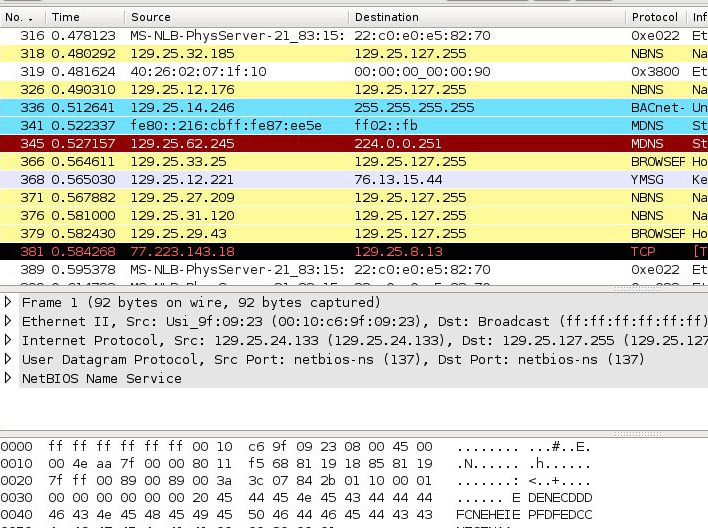
\includegraphics[width=.75\textwidth]{gfx/wireshark}
    \end{figure}
    \begin{itemize}
        \item Find packets related to service with Wireshark/TCPDump/etc.
    \end{itemize}
    \note[item]{Tom}
\end{frame}

%------------------------------------------------------------------------------

\begin{frame}[fragile,allowframebreaks]{Manual Process}
    \begin{itemize}
        \item Need to find API for web service.
        \item Need to examine payloads from invocations and try to guess API.
        \item Once this is done (hard), need to write WSDL by hand.
    \end{itemize}
    \begin{lstlisting}
<?xml version="1.0" encoding="UTF-8"?>
<definitions name="DayOfWeek" targetNamespace="..." xmlns:tns="..." xmlns:soap="..." xmlns:xsd="..." xmlns="..."> 
  <message name="DayOfWeekInput">
    <part name="date" type="xsd:date"/>
  </message>
  <message name="DayOfWeekResponse">
    <part name="dayOfWeek" type="xsd:string"/>
  </message>
  <portType name="DayOfWeekPortType">
    <operation name="GetDayOfWeek">
      <input message="tns:DayOfWeekInput"/>
      <output message="tns:DayOfWeekResponse"/>
    </operation>
  </portType>
  <binding name="DayOfWeekBinding" type="tns:DayOfWeekPortType">
    <soap:binding style="document" 
      transport="http://schemas.xmlsoap.org/soap/http"/>
    <operation name="GetDayOfWeek">
      <soap:operation soapAction="getdayofweek"/>
      <input>
        <soap:body use="encoded" 
          namespace="http://www.roguewave.com/soapworx/examples" 
          encodingStyle="http://schemas.xmlsoap.org/soap/encoding/"/>
      </input>
      <output>
        <soap:body use="encoded" 
          namespace="http://www.roguewave.com/soapworx/examples"  
          encodingStyle="http://schemas.xmlsoap.org/soap/encoding/"/>
      </output>
    </operation>
  </binding>
  <service name="DayOfWeekService">
    <documentation>
      Returns the day-of-week name for a given date
    </documentation>
    <port name="DayOfWeekPort" binding="tns:DayOfWeekBinding">
      <soap:address location="http://localhost:8090/dayofweek/DayOfWeek"/>
    </port>
  </service>
</definitions>
    \end{lstlisting}
    \begin{itemize}
        \item This is not fun.
        \item Computers can do this for you!
    \end{itemize}
    \note[item]{Tom}
\end{frame}

%------------------------------------------------------------------------------

\subsection{Using ServiceSniffer}
\begin{frame}{Using ServiceSniffer}
    \framesubtitle{Main Screen}
    % From: http://www.texample.net/tikz/examples/connecting-text-and-graphics/
    \begin{tikzpicture}
        \node [inner sep=0pt,above right]
            {\includegraphics[width=.95\textwidth]{gfx/gui-main}};
        % define destination coordinates
        % \fill (6.8,5.8) circle (2pt);
        \path (1.5,4) coordinate (list)
              (6.8,5.8) coordinate (udditab);
    \end{tikzpicture}
    \only<2>{List of all detected services \tikz[na] \coordinate (listpt);}
    \only<3>{Click to access UDDI registry \tikz[na] \coordinate (uddipt);}
    \begin{tikzpicture}[overlay]
        \path <2> [->,red,thick] (listpt) edge [bend right] (list);
        \path <3> [->,red,thick] (uddipt) edge [bend left] (udditab);
    \end{tikzpicture}
    \note[item]{Tom}
\end{frame}

%------------------------------------------------------------------------------

\begin{frame}{Using ServiceSniffer}
    \framesubtitle{UDDI Registry}
    \begin{tikzpicture}
        \node [inner sep=0pt,above right]
            {\includegraphics[width=.95\textwidth]{gfx/gui-uddi}};
        % define destination coordinates
        %\fill (1.2,.8) circle (2pt);
        \path (1.5,5) coordinate (tree)
              (4,4.5) coordinate (general)
              (5.1,5.4) coordinate (source)
              (1.3,.8) coordinate (add);
    \end{tikzpicture}
    \only<2>{
        \begin{itemize}
            \vspace{-4mm}
            \item Top level is hosts \tikz[na] \coordinate (uddipt);
            \item 2nd level is individual service
            \item 3nd level are port bindings
        \end{itemize}
    }
    \only<3>{General information about particular host \tikz[na] \coordinate (generalpt);}
    \only<4>{Manually add/remove entries \tikz[na] \coordinate (addpt);}
    \only<5>{UDDI registry entry\tikz[na] \coordinate (sourcept);}
    \begin{tikzpicture}[overlay]
        \path <2> [->,red,thick] (uddipt) edge [bend right] (tree);
        \path <3> [->,red,thick] (generalpt) edge [bend right] (general);
        \path <4> [->,red,thick] (addpt) edge [bend right] (add);
        \path <5> [->,red,thick] (sourcept) edge [bend right] (source);
    \end{tikzpicture}
    \note[item]{Tom}
\end{frame}

%------------------------------------------------------------------------------

\begin{frame}{Using ServiceSniffer}
    \framesubtitle{UDDI Registry}
    \begin{tikzpicture}
        \node [inner sep=0pt,above right]
            {\includegraphics[width=.95\textwidth]{gfx/gui-uddi2}};
    \end{tikzpicture}
    Able to export source to other programs.
    \note[item]{Tom}
\end{frame}

%------------------------------------------------------------------------------

\begin{frame}{Using ServiceSniffer}
    \framesubtitle{Service Properties}
    \begin{tikzpicture}
        \node [inner sep=0pt,above right]
            {\includegraphics[width=.95\textwidth]{gfx/gui-properties}};
    \end{tikzpicture}
    Also, see detailed information on particular service
    \note[item]{Tom}
\end{frame}

%------------------------------------------------------------------------------
%
%\subsection{Design Overview}
%\begin{frame}{Design}
%    \tikzstyle{entity} = [top color=white, bottom color=blue!30,
%        draw=blue!50!black!100, drop shadow]
%    \tikzstyle{line} = [draw, -latex']
%    \tikzstyle{highlight} = [fill=yellow!40,rounded corners]
%    \pgfdeclarelayer{background layer}
%    \pgfdeclarelayer{highlight layer}
%    \pgfsetlayers{background layer,highlight layer,main}
%    \begin{tikzpicture}[node distance=3cm, auto]
%        \node [entity] (capture) {Capture};
%        \node [entity] (pcap1) [above left of=capture] {PCAP File};
%        \node [cloud, cloud ignores aspect, cloud puffs=20, top color=white, bottom color=blue!30, draw=blue!50!black!100, drop shadow]
%            (network) [below left of=capture] {Network};
%        \node [entity] (pcap2) [above of=capture] {PCAP File};
%        \node [entity] (kernel) [right of=capture] {System Kernel};
%        \node [entity] (filters) [above of=kernel] {Filters};
%        \node [entity] (processors) [above right of=kernel] {Processors};
%        \node [entity] (gui) [below left of=kernel] {GUI};
%        \node [entity] (cli) [below right of=kernel] {CLI};
%
%        % This is to keep the figure from shifting around when we draw the highlights
%        \node [use as bounding box,fit=(capture)(pcap1)(network)(pcap2)(kernel)(filters)(processors)(gui)(cli)] {};
%
%        % Edges
%        \draw [->] (pcap1) |- (capture);
%        \draw [->] (network) |- (capture);
%        \draw [->] (capture) -- (pcap2);
%        \draw [->] (capture) -- (kernel);
%        \draw [<->] (kernel) -- (filters);
%        \draw [<->] (kernel) -| (processors);
%        \draw [<->] (kernel) |- (gui);
%        \draw [<->] (kernel) |- (cli);
%
%        % Background
%        \begin{pgfonlayer}{background layer}
%            \node [fill=black!30,rounded corners,fit=(capture)(kernel)(filters)(processors)] {};
%        \end{pgfonlayer}
%        
%        % Highlights
%        \begin{pgfonlayer}{highlight layer}
%            \node <2> [highlight,fit=(pcap1)(pcap2)(capture)(network)] {};
%            \node <3> [highlight,fit=(kernel)] {};
%            \node <4> [highlight,fit=(filters)(processors)] {};
%            \node <5> [highlight,fit=(gui)(cli)] {};
%        \end{pgfonlayer}
%    \end{tikzpicture}
%\end{frame}
%
%------------------------------------------------------------------------------

\begin{frame}{Design Overview}
    \begin{figure}
        \vspace{-2em}
        \centering
        \includegraphics[width=.75\textwidth]{gfx/dataflow_base}
        \vspace{-3em}
    \end{figure}
    \begin{itemize}
        \item{Four main section of the system:}
        \begin{multicols}{2}
            \begin{itemize}
                \item{Input}
                \item{System Kernel}
                \item{Filters and Processing}
                \item{Interfaces}
            \end{itemize}
        \end{multicols}
    \end{itemize}
    \note[item]{Charles}
\end{frame}

%------------------------------------------------------------------------------

\begin{frame}{Design Overview}
    \framesubtitle{System Input}
    \begin{figure}
        \vspace{-2em}
        \centering
        \includegraphics[width=.75\textwidth]{gfx/dataflow_input}
        \vspace{-3em}
    \end{figure}
    \begin{itemize}
        \item{Uses LibPCAP}
        \item{Ability to process live network traffic and Pcap files}
        \item{Ability to dump live network traffic for later processing}
    \end{itemize}
    \note[item]{Charles}
\end{frame}

%------------------------------------------------------------------------------

\begin{frame}{Design Overview}
    \framesubtitle{System Kernel}
    \begin{figure}
        \vspace{-2em}
        \centering
        \includegraphics[width=.75\textwidth]{gfx/dataflow_kernel}
        \vspace{-3em}
    \end{figure}
    \begin{itemize}
        \item{Centeral core to the system}
        \item{Control flow of information to the rest of the system}
        \item{Interacts with input, processing and interfaces}
    \end{itemize}
    \note[item]{Charles}
\end{frame}

%------------------------------------------------------------------------------

\begin{frame}{Design Overview}
    \framesubtitle{Filters and Processing}
    \begin{figure}
        \vspace{-2em}
        \centering
        \includegraphics[width=.75\textwidth]{gfx/dataflow_processing}
        \vspace{-3em}
    \end{figure}
    \begin{itemize}
       \item{Ability to reduce the data being shown or processing}
       \item{Processors can determine useful information from web services}
    \end{itemize}
    \note[item]{Charles}
\end{frame}

%------------------------------------------------------------------------------

\begin{frame}{Design Overview}
    \framesubtitle{Interfaces}
    \begin{figure}
        \vspace{-2em}
        \centering
        \includegraphics[width=.75\textwidth]{gfx/dataflow_output}
        \vspace{-3em}
    \end{figure}
    \begin{itemize}
        \item{User control of the system}
        \item{Ability to control filters and processors}
        \item{Allows for different interfaces}
    \end{itemize}
    \note[item]{Charles}
\end{frame}

%------------------------------------------------------------------------------

\subsection{Extensibility}
\begin{frame}{Extensibility}
    \begin{itemize}
        \item New protocols --- XMPP / Hessian or non-web service protocols
        \item New reports --- Custom aggregate data
        \item New interfaces --- Mobile Client / Facebook App
        \item New filters --- Protocol specific filters
        \item New processors --- Protocol specific processors
    \end{itemize}
    \note[item]{Phil}
\end{frame}

%------------------------------------------------------------------------------

\section{Conclusions}
\subsection{Preliminary Results}
\begin{frame}{Preliminary Results}
    \begin{itemize}
        \item PCAP in Python --- 10M packets / 6GB : 4 seconds
        \item UNIX Socket --- Language agnostic processors / filters
    \end{itemize}
    \note[item]{Phil}
\end{frame}

%------------------------------------------------------------------------------

\subsection{System Evolution}
\begin{frame}{System Evolution}
    \begin{itemize}
        \item New report screens
        \item Multiple ServiceSniffer registries merge
        \item Distributed live capture and analysis
    \end{itemize}
    \note[item]{Justin}
\end{frame}

%------------------------------------------------------------------------------

\subsection{Questions}
\begin{frame}{Questions?}
    \begin{itemize}
        \item See our website at \url{http://servicesniffer.net}
        \item Can send questions to \url{list@servicesniffer.net}
    \end{itemize}
    \note[item]{Justin}
\end{frame}

\end{document}
